Mit den Teilgeschwindigkeiten $v_x = v_0\cos\alpha$ und $v_y = v_0\sin\alpha$ ist die Bahn (Abwurf im Ursprung, nach oben positiv)
\begin{align}
 x(t) &= v_0\cos\alpha\cdot t \\
 y(t) &= v_0\sin\alpha\cdot t - \frac{1}{2}g\,t^2
\end{align}
Eliminiert man $t = x/(v_0\cos\alpha)$, so erhält man die Wurfparabel
\begin{align}
 y(x) &= \tan\alpha\cdot x - \frac{g}{2v_0^2\cos^2\alpha}\cdot x^2
\end{align}
Der Ball ist wieder auf der Abwurfhöhe ($y = 0$) nach der Flugzeit $t = 2v_0\sin\alpha/g$. Die Wurfweite ist deshalb
\begin{align}
 w &= v_0\cos\alpha\cdot\frac{2v_0\sin\alpha}{g} = \frac{2v_0^2\sin\alpha\cos\alpha}{g} = \frac{v_0^2}{g}\,\sin(2\alpha)
\end{align}
Bei fester Abwurfgeschwindigkeit $v_0$ hängt $w$ nur über $\sin(2\alpha)$ vom Winkel ab. Der Sinus ist am grössten (gleich 1) für $2\alpha = \ang{90}$, also für
\begin{align}
 \alpha &= \result{\ang{45}}, \qquad w_\text{max} = \frac{v_0^2}{g}
\end{align}
Wegen $\sin(2\alpha) = \sin(\ang{180}-2\alpha)$ ergeben die Winkel $\alpha$ und $\ang{90}-\alpha$ dieselbe Wurfweite (z.B. $\ang{30}$ und $\ang{60}$), die steilere Bahn ist aber höher und dauert länger.

Die Abbildung zeigt die Wurfparabeln für $\alpha = \ang{15}, \ang{30}, \ang{45}, \ang{60}, \ang{75}$ bei gleichem $v_0$ (Achsen in Einheiten von $v_0^2/g$):
\begin{center}
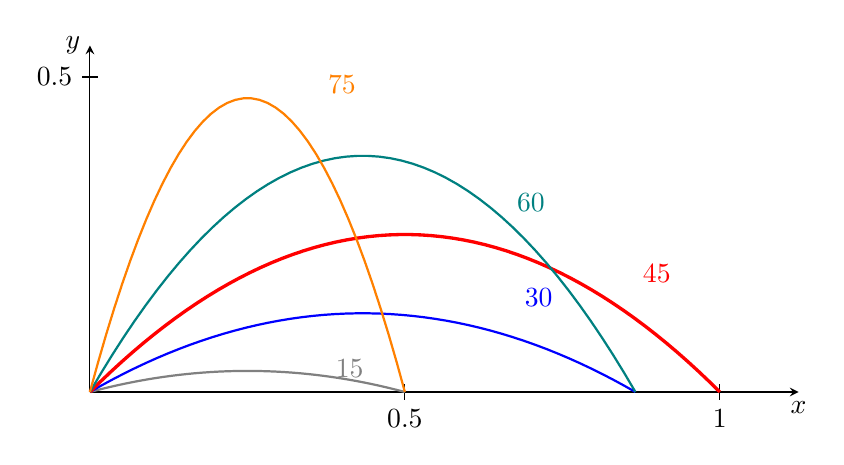
\begin{tikzpicture}[>=stealth, scale=1]
 \draw[->] (0,0) -- (9,0) node[below] {$x$};
 \draw[->] (0,0) -- (0,4.4) node[left] {$y$};
 \draw (8,0.1) -- (8,-0.1) node[below] {$1$};
 \draw (4,0.1) -- (4,-0.1) node[below] {$0.5$};
 \draw (0.1,4) -- (-0.1,4) node[left] {$0.5$};
 \draw[thick, gray, domain=0:4, samples=40] plot (\x, {\x*tan(15)-\x*\x/(16*cos(15)^2)});
 \draw[thick, blue, domain=0:6.928, samples=50] plot (\x, {\x*tan(30)-\x*\x/(16*cos(30)^2)});
 \draw[very thick, red, domain=0:8, samples=60] plot (\x, {\x*tan(45)-\x*\x/(16*cos(45)^2)});
 \draw[thick, teal, domain=0:6.928, samples=50] plot (\x, {\x*tan(60)-\x*\x/(16*cos(60)^2)});
 \draw[thick, orange, domain=0:4, samples=40] plot (\x, {\x*tan(75)-\x*\x/(16*cos(75)^2)});
 \node[gray, anchor=west] at (3.0,0.3) {$\ang{15}$};
 \node[blue, anchor=west] at (5.4,1.2) {$\ang{30}$};
 \node[red, anchor=west] at (6.9,1.5) {$\ang{45}$};
 \node[teal, anchor=west] at (5.3,2.4) {$\ang{60}$};
 \node[orange, anchor=west] at (2.9,3.9) {$\ang{75}$};
\end{tikzpicture}
\end{center}
Die $\ang{45}$-Parabel reicht am weitesten; die Paare $\ang{30}$/$\ang{60}$ und $\ang{15}$/$\ang{75}$ landen jeweils am gleichen Ort.
